\documentclass{beamer}
\usepackage{ctex}
% \usepackage{CJKutf8}
% \usepackage{xeCJK}
\usepackage{fontspec}
\usepackage[]{geometry}

% \usepackage{CJKutf8}    % encode for Chinese
\usepackage{times}      % font for english, Times New Roman
\usepackage{amsmath, amsfonts, amssymb} % math equations, symbols
\usepackage[english]{babel}
\usepackage{color}      % color content
\usepackage{graphicx}   % import figures
\usepackage{url}        % hyperlinks
\usepackage{bm}         % bold type for equations
\usepackage{hyperref}   % bookmarks
% \hypersetup{bookmarks, unicode} % unicode

\usetheme{Madrid}


%Information to be included in the title page:
\title{数学物理方法}
\author{罗凯}
\institute{南京理工大学理学院}
\date{2023年}

\begin{document}
% \begin{CJK}{UTF8}{song}

\AtBeginSection[]
{

% \begin{frame}
%     \tableofcontents[currentsection,hideallsubsections]
% \end{frame}

% \begin{frame}
%    	\ftitle{Outline 目录}		% contents for better review
%     \tableofcontents[currentsection, currentsubsection]
% \end{frame}
\begin{frame}[shrink]
    \tableofcontents[sectionstyle=show/shaded,subsectionstyle=show/shaded/hide]
\end{frame}
}



\begin{frame}
    \titlepage	% make the cover page here
\end{frame}


% \part{复变函数论}

\chapter{复变函数论}
\label{chap:complexfunctions}
复变函数论是物理学和工程学广泛使用的强大分析工具,学习掌握这个理论十分必要。

\section{复数和复变函数}



\subsection{复数的定义}
一元二次方程$a x^2 + b x + c = 0 (a\neq 0, b,c \in \mathbb{R})$的求解大家一定都不陌生。当$\Delta \equiv b^2 - 4 a c \geq 0$时,方程有解,求根公式可得
\begin{equation}
    x = \frac{-b \pm \sqrt{\Delta}}{2a} 。
\end{equation}
当$\Delta < 0$时,方程无解。这里的无解其实是指没有实数解。
当我们引入以下这一核心定义后,
\begin{equation}
    \imath ^2 = -1 \quad \textrm{或} \quad \imath = \sqrt{-1} 。 
\end{equation}
$\imath$为{\bf 虚数},将定义域扩展到复数,二次方程就有确定的两个解,当$\Delta < 0$时,方程有两个复数解:
\begin{equation}
    x = \frac{-b \pm \imath \sqrt{-\Delta}}{2a} 。
\end{equation}
复数$z$定义为
\begin{equation}
    \label{eq:complex_alg}
    z = x + \imath \; y ,
\end{equation}
$x,y \in {\mathbb{R}}$。$x,y$分别为复数$z$的{\bf 实部}(real part) 和{\bf 虚部}(imaginary part),分别记作$\Re z$和$\Im z$。
上式\eqref{eq:complex_alg}成为复数的代数式。复数域常用$\mathbb{C}$来表示。若将$z$看成是由$x,y$组成的有序对$(x,y)$,记为
\begin{equation}
    z \equiv (x,y),
\end{equation}
则有$1 = (1,0), \imath = (0, 1)$。如果将$x,y$当做平面上点的坐标,复数$z$就和平面上的点一一对应起来。
形成的平面叫做{\bf 复数平面},坐标轴成为{\bf 实轴}和{\bf 虚轴}。
\begin{figure}[htb]
    \centering
    \begin{tikzpicture}[scale=1.5]
    \path (0,0) coordinate (origin);
    \path (4, 0) coordinate (x) ;
    \path (0, 2.5) coordinate (y) ;
    \path (4, 2.5) coordinate (z);
    \path (2.5, 2) coordinate (rho);
  
    \draw[->] (-0.2,0) --(4.2,0) node[right] {$\Re$};
    \draw[->] (0,-0.2) --(0,3.2) node[above] {$\Im$};
    \draw[solid, text=blue, thick, -{Stealth[length=2mm]}] (origin) -- (z) node[above] {$z=\rho e^{\imath \varphi}$};
    \draw[text=red, dashed]  (x) --(z) node[above]  {};
    \draw[text=red, dashed] (y) --(z) node[above] {};
  
    \node at (origin) [below] {$O$};
    \node at (x) [below ]{$x$};
    \node at (y) [left ]{ $y$};
    \node at (rho) [right] {$\rho$};
    \draw[color=red, fill=red] (z) circle (0.05);
  
    \draw pic["$\varphi$",draw, ->, angle eccentricity=1.2, angle radius=0.8cm]{angle = x--origin--z};
  
  \end{tikzpicture}
  \caption{复数的平面表示。} \label{fig:complex_plane}
\end{figure} 
自然我们可以改用极坐标来表示,
\begin{align}
    & \rho = \sqrt{x^2 + y^2}\\
    & \varphi = \arctan y/x
\end{align}
或
\begin{align}
    & x = \rho \cos\varphi \\
    & y = \rho \sin\varphi 
\end{align}
则我们得到复数$z$的三角式
\begin{equation}
    z = \rho (\cos\varphi +  \imath\; \sin\varphi) ,
\end{equation}
或指数式
\begin{equation}
    z = \rho e^{\imath \varphi} 。
\end{equation}
$\rho = |z|$ 为复数的{\bf 模}(modulus), $\varphi$为复数的{\bf 辐角}(argument),记作$\Arg z$。
对于任意一个$z=\rho e^{\imath \varphi}$,由于恒等式$e^{\imath 2\pi n} = 1$, $n = 0, \pm 1, \pm 2, \dots, \in \mathbb{Z}$,
可以知道辐角$\Arg z$不能唯一确定,它们之间相差$2\pi$的整数倍,其中满足
\begin{align}
    0 \leq \Arg z < 2\pi ,
\end{align}
的辐角为$z$的主辐角,记为$\arg z$。$\arg z$ 为$\Arg z$的主值。
\begin{align}
    \Arg z = \arg z + 2 n \pi \quad (n = 0, \pm 1, \pm 2\dots)。
\end{align}


\begin{example}
求$\sqrt[3]{-\imath}$。
\end{example}
\begin{solution}

\begin{minipage}{0.7\textwidth}
    首先,我们有恒等式$e^{\imath 2\pi n} = 1$,且
    \begin{align*}
        e^{\imath \frac{\pi}{2}}  = i & \quad  e^{\imath \pi}  =-1 \\
        e^{\imath \frac{3\pi}{2}} = -i & \quad e^{\imath 2\pi} = 1。
    \end{align*}
题目就是要求方程$z^3 =-\imath$的根。可以得到
    \begin{align*}
        e^{\frac{1}{3}(\imath 2\pi n + \imath \frac{3\pi}{2})} & = (-i)^{\frac{1}{3}} \\
        e^{(\imath \frac{2}{3}\pi n + \imath \frac{\pi}{2})}   & =  (-i)^{\frac{1}{3}} \\
    \end{align*}
得到的解分三种情况
    \begin{align*}
        z_1 &=e^{\imath \frac{\pi}{2}} = \imath , n = 3k \\
        z_2 &=e^{\imath \frac{7\pi}{6}} = -\frac{\sqrt{3}}{2} - \frac{\imath}{2} , n = 3k +1 \\
        z_3 &=e^{\imath \frac{11\pi}{6}} = \frac{\sqrt{3}}{2} - \frac{\imath}{2} , n = 3k +2 
    \end{align*}
它们在复平面上的分布如下图所示,它们之间的夹角为$120^\circ$,模为单位长度$1$。
    % \begin{figure}
\end{minipage}
\begin{minipage}{0.3\textwidth}
    % \begin{figure} 
        \begin{tikzpicture}[scale=1.5]
    \def\sin60{}
    \path (0,0) coordinate (origin);
    \path (0, 1) coordinate (z1) ;
    \path ({-sqrt(3)/2}, -0.5 ) coordinate (z2) ;
    \path ({sqrt(3)/2},  -0.5) coordinate (z3);
  
    \draw[->] (-1.5,0) --(1.5,0) node[right] {$\Re$};
    \draw[->] (0,-1.5) --(0,1.5) node[above] {$\Im$};
    \draw[dashed, text=blue, thick, -{Stealth[length=2mm]}] (origin) -- (z1) node[above,right] {$z_1$};
    \draw[dashed, text=blue, thick, -{Stealth[length=2mm]}] (origin) -- (z2) node[below] {$z_2$};
    \draw[dashed, text=blue, thick, -{Stealth[length=2mm]}] (origin) -- (z3) node[below] {$z_3$};
    % \draw[text=red, dashed] (y) --(z) node[above] {};
  
    % \node at (origin) [left] {$O$};
    % \node at (rho) [right] {$\rho$};
    \draw[color=red, dashed] (origin) circle (1);
    % \draw
    \draw[color=red, fill=red] (z1) circle (0.05);
    \draw[color=red, fill=red] (z2) circle (0.05);
    \draw[color=red, fill=red] (z3) circle (0.05);
    % \draw pic["$\varphi$",draw, ->, angle eccentricity=1.2, angle radius=0.8cm]{angle = x--origin--z};
    % \draw pic["$\varphi$",draw, <-, angle eccentricity=1.2, angle radius=0.8cm]{angle = zminus--origin--x};

  \end{tikzpicture}
        % \caption{$\sqrt[3]{-\imath}$的三个根示意图。}
    % \end{figure}
\end{minipage}

\end{solution}

\subsection{复数的运算}
我们可以利用有序实数对的方式对复数进行基本运算: 加减乘除运算。{\bf 加法}运算可以定义为
\begin{align}
    z_1 + z_2 = (x_1, y_1) + (x_2, y_2) = (x_1 + x_2, y_1 + y_2) 。
\end{align}
{\bf 乘法}运算定义为
\begin{align}
    z_1 \cdot z_2 = (x_1, y_1) \cdot (x_2, y_2) = (x_1 x_2 - y_1 y_2, x_1 y_2 + x_2 y_1) 。
\end{align}
显然加法和乘法满足{\bf 交换律}和{\bf 结合律},以后乘法运算符号$\cdot$均省略。
同实数一样,根据以上定义我们可以得到复数域中的一些特殊元素。对于任意复数$z$,复数域中存在元素$e$满足以下性质
\begin{align}
    & e + z = z + e = z ,\\ 
    & e \cdot z = z \cdot e = z , 
\end{align}
可以得到对应的分别为
\begin{align}
    (0, 0) &= 0\\
    (1, 0) &= 1 ,
\end{align}
通过元素$(0,0)$,我们可以定义$-z$使得 $-z + z = 0$。 于是有,$- z = (-x, -y)$。于是我们定义
{\bf 减法}运算为 
\begin{align}
    z_1 - z_2 \equiv z_1 + (-z_2) = (x_1 - x_2, y_1 - y_2) ,
\end{align}
通过元素$(1,0)$,我们定义$z^{-1}$使得
$z^{-1} \cdot z = 1$,于是有 $z^{-1} =e^{-\imath \varphi}/\rho  $。
或$z^{-1} = (\frac{x}{x^2 + y^2}, -\frac{y}{x^2 + y^2})$。{\bf 除法}运算定义为
\begin{align}
    z_1 / z_2 \equiv z_1 \cdot z_2^{-1} = \frac{x_1 x_2 - y_1 y_2} {x_2^2  +  y_2^2 }  + \imath \frac{y_1 x_2 - x_1 y_2} {x_2^2  +  y_2^2 } 。 
\end{align}
注意往往乘除写成极坐标表达更简洁:
\begin{align}
    z_1 z_2 = \rho_1 e^{\imath \varphi_1 } \rho_2 e^{\imath \varphi_2 } = \rho_1 \rho_2 e^{\imath (\varphi_1 + \varphi_2)}
\end{align}

此外,复数还有一种运算较为特殊,称为{\bf 共轭}(complex conjugation)运算。共轭运算表示为
\begin{align}
    z^{*} \equiv (x, -y) = x - \imath y ,
\end{align}
也记为$\bar{z}$。
实部虚部可以通过
\begin{equation}
    \operatorname{Re} a=\frac{a+\bar{a}}{2}, \quad \operatorname{Im} a=\frac{a-\bar{a}}{2 \mathrm{i}}
\end{equation}
复数和其共轭来表示。不难验证

\begin{equation}
    \begin{aligned}
    & \overline{a+b}=\bar{a}+\bar{b} \\
    & \overline{a b}=\bar{a} \bar{b}
    \end{aligned}
\end{equation}

作为应用, 考虑方程
$$
c_0 z^n+c_1 z^{n-1}+\cdots+c_{n-1} z+c_n=0 。
$$
如果 $\zeta$ 是这个方程的一个根, 则 $\bar{\zeta}$ 是方程
$$
\bar{c}_0 z^n+\bar{c}_1 z^{n-1}+\cdots+\bar{c}_{n-1} z+\bar{c}_n=0 。
$$
的根。 特别地, 如果系数为实数, 则 $\zeta$ 和 $\bar{\zeta}$ 是同一方程的根, 
而且我们得到定理:实系数方程的非实根以成对的共轭根出现。

为了得到$z$的模,我们可以利用共轭运算,$|z| = \sqrt{zz^{*}}$。注意区分$|z|^2$和$z^2$的不同。

部分复数运算可以映射到复平面上。如共轭运算可以理解为对$z$以实轴为对称轴的镜面对称。对任意的$z_1,z_2$,它们的加减
同向量的加减完全等价,由三角形的三边关系可得
\begin{equation}
    \left| |z|- |z'| \right| \leq |z \pm z'| \leq |z| + |z'| 。
\end{equation}
% 很显然,$z+z^{*} = 2 \Re z$, $z-z^{*} = 2\imath \Im z$。
\begin{figure}[h]
% \begin{minipage}{0.5\textwidth}
% \begin{figure}[htb]
    \centering
    \begin{tikzpicture}[scale=0.8]
    \path (0,0) coordinate (origin);
    \path (4, 0) coordinate (x) ;
    \path (0, 2.5) coordinate (y) ;
    \path (3, 2.0) coordinate (z);
    \path (3,-2.0) coordinate (zminus);
    % \path (2.5, 2) coordinate (rho);
  
    \draw[->] (-0.2,0) --(4.2,0) node[right] {$\Re$};
    \draw[->] (0,-2.5) --(0,2.5) node[above] {$\Im$};
    \draw[solid, text=blue, thick, -{Stealth[length=2mm]}] (origin) -- (z) node[above] {$z=\rho e^{\imath \varphi}$};
    \draw[solid, text=blue, thick, -{Stealth[length=2mm]}] (origin) -- (zminus) node[below] {$z^{*}=\rho e^{-\imath \varphi}$};
    \draw[text=red, dashed]  (zminus) --(z) node[above]  {};
    % \draw[text=red, dashed] (y) --(z) node[above] {};
  
    \node at (origin) [left] {$O$};
    \node at (x) [below ]{$x$};
    \node at (y) [left ]{ $y$};
    % \node at (rho) [right] {$\rho$};
    \draw[color=red, fill=red] (z) circle (0.05);
    \draw[color=red, fill=red] (zminus) circle (0.05);
    % \draw pic["$\varphi$",draw, ->, angle eccentricity=1.2, angle radius=0.8cm]{angle = x--origin--z};
    % \draw pic["$\varphi$",draw, <-, angle eccentricity=1.2, angle radius=0.8cm]{angle = zminus--origin--x};

  \end{tikzpicture}
%   \caption{共轭的几何表示.} \label{fig:zminus}
% \end{figure} 
% \end{minipage}
\quad 
% \begin{minipage}{0.5\textwidth}
    % \begin{figure}[htb]
        % \centering
        \begin{tikzpicture}[scale=0.8]
    % Define the vectors
    \path (3, 2.0) coordinate (z1);
    \path (1, -1.0) coordinate (z2);
    \path (4, 1) coordinate (z1pz2);
    \path (2, 3) coordinate (z1mz2);

    \draw[-{Stealth[length=2mm]}] (0,0) -- (z1) node[midway, above]{$z_1$};
    \draw[-{Stealth[length=2mm]}] (0,0) -- (z2) node[left]{$z_2$};
    % Draw the vector addition
    \draw[-{Stealth[length=2mm]}, text=blue, thick] (0,0) -- (z1pz2) node[midway, below]{$z_1 + z_2$};
    \draw[-{Stealth[length=2mm]}, text=blue, dashed] (z1) -- (z1pz2) node[midway, right]{$z_2$};

    % Draw the vector subtraction
    \draw[-{Stealth[length=2mm]}, text=blue, thick] (0,0) -- (z1mz2) node[midway, left]{$z_1 - z_2$};
    \draw[-{Stealth[length=2mm]}, text=blue, dashed] (z1) -- (z1mz2) node[midway, right]{$- z_2$};
    \path (0,0) coordinate (origin);
  
    \draw[->] (-0.2,0) --(4.2,0) node[right] {$\Re$};
    \draw[->] (0,-2.5) --(0,2.5) node[above] {$\Im$};
    \node at (origin) [left] {$O$};

  \end{tikzpicture}
    %   \caption{共轭的几何表示.} \label{fig:zminus}
    % \end{figure} 
% \end{minipage}
        \caption{左图:共轭$z^{*}$与$z$的关系; 右图:$z_1, z_2$的加减关系。}
\end{figure}
 

\begin{example}
讨论$\Re \frac{1}{z} = 2$在复平面上的意义。
\end{example}
\begin{solution}
    \begin{align*}
        \Re \frac{1}{z} &= 2\\
        \Re \frac{1}{x+\imath y} &  = 2 \\
        \frac{x}{x^2 +y^2} & = 2 。
    \end{align*}
因此,我们得到方程
\[
    (x-\frac{1}{4})^2 + y^2 = \left( \frac{1}{4}\right)^2,
\]
它表示以$(\frac{1}{4},0)$为圆心,$\frac{1}{4}$为半径的圆上各点集合。
\end{solution}
        

\begin{note}
    挑战自我: 试证明点 $a_1, a_2, a_3$ 当且仅当 
    $a_1^2+a_2^2+a_3^2=a_1 a_2+a_2 a_3+a_3 a_1$ 时为等边三角形的三个顶点。    
\end{note}
% \subsection{复数运算的几何表示}




% \subsubsection{}
\subsection{复变函数}
\label{sub:complexfunctions}

\subsubsection{定义}
\label{subsub:cmplx_func_def}

存在复数平面的点集$Z$,每一点$z\in Z$有一个或多个复数值$w$与之对应,则称$w$为$z$的函数--复变函数。$z$称为$w$的宗量,定义域为$Z$,记作
\begin{equation}
    w = w(z)\textrm{,} z\in Z \textrm{。}
\end{equation}
任意一个复变函数$w(z)$,$z=x + \imath y$,我们可以写称实部和虚部的组合,
\begin{align}
    w(z) = u(x,y) +\imath \; v(x,y) \textrm{,}
\end{align}
其中$u(x,y), v(x,y)$为纯实函数。它们可以类似的写成
\begin{align}
    \Re w(z) = u(x,y)\textrm{,} \quad \Im w(z) = v(x,y) \textrm{,}
\end{align}
$w(z)$的复共轭为$u(x,y) - \imath \; v(x,y)$。取决于$w(z)$,二者可能相等也可能不等。

这里我们列举一些常见复变函数。
\begin{itemize}
    \item 多项式:
        \begin{equation}
            a_0 + a_1 z + a_2 z^2 + \cdots + a_n z^n \textrm{,} \quad n\in \mathbb{Z}^+ \textrm{,}
        \end{equation}
    \item 有理分式:       
         \begin{equation}
        \frac{a_0 + a_1 z + a_2 z^2 + \cdots + a_n z^n}{{b_0 + b_1 z + b_2 z^2 + \cdots + b_m z^m}} \textrm{,} \quad  n,m\in \mathbb{Z}^+ \textrm{,}
        \end{equation}
    \item 根式:
        \begin{equation}
            (z-a)^{m/n} \textrm{,} \quad  n,m\in \mathbb{Z}^+ \textrm{,}
        \end{equation}
    \item 对数、指数
        \begin{equation}
            \ln z = \ln |z| + \imath \Arg z, \quad z^s = e^{s\ln z} \textrm{,}
        \end{equation}
    \item 正余弦,正余切函数 
        \begin{equation}
            \sin z , \cos z , \tan z, \cot z \textrm{,}
        \end{equation}
    \item 双曲正余弦, 双曲正余切函数
        \begin{equation}
            \sinh z , \cosh z , \tanh z, \coth z  \textrm{。}
        \end{equation}
\end{itemize}
以上所有出现的常数均为复数。

\begin{examplebox}{验证\begin{equation*}
    |\sin z|=\frac{1}{2} \sqrt{\left(e^{2 y}+e^{-2 y}\right)+2\left(\sin ^2 x-\cos ^2 x\right)} .
    \end{equation*}
    }
    由正弦函数定义得
    \begin{align*}
        \sin z &= \frac{e^{\imath z} - e^{-\imath z}}{2\imath} 
        \\ 
        & = \frac{e^{\imath x - y} - e^{-\imath x + y}}{2\imath}
        \\
        & = \frac{1}{2\imath}\left( e^{-y} (\cos x + \imath \sin x ) - e^{y} (\cos x - \imath \sin x ) \right) 
        \\
        & = \frac{1}{2\imath} \left( \cos x (e^{-y} - e^{y}) + \imath \sin x (e^{-y} + e^{y}) \right)
    \end{align*}
    取模后可得,
    \begin{align*}
        |\sin z | &= \frac{1}{2}\sqrt{ \cos^2x (e^{2y} + e^{-2y} -2) + \sin^2 x (e^{2y} + e^{-2y} +2) }
        \\
        &=\frac{1}{2}\sqrt{\left(e^{2 y}+e^{-2 y}\right)+2\left(\sin ^2 x-\cos ^2 x\right)}
    \end{align*}
    可见,与实函数不同的是,$|\sin z|$的取值完全可以大于$1$。
\end{examplebox}

复数
\begin{figure}
    \centering

    \input{tikz/branch_cut.tex}

\end{figure}
\section{解析函数}
\chapter{定积分的计算}
对于实变函数的定积分,我们已经学会了一些积分技巧,如变量代换,分部积分等.这一章我们将介绍利用留数定理的积分技巧,并介绍以物理学家Richard P. Feynman命名的
特殊技巧.

\section{留数定理应用}
\subsection{三角函数的积分}
考虑积分区间为$\left[ 0, 2\pi \right]$,被积函数为三角函数有理式的积分
\begin{equation}
    \int_{0}^{2\pi} R(\cos{x}, \sin{x}) dx,
\end{equation}
当实变数 $x$ 从 0 变到 $2 \pi$ 时, 复变数 $z=e^{\imath x}$ 从 $z=1$ 出发沿单位圆 $|z|=1$ 逆时针 走一圈又回到 $z=1$,
实变定积分化为复变回路积分, 就可以应用留数定理了. 至于实变定积分里的 $\cos x, \sin x$ 和 $d x$, 作如下变换:
$$
\cos x=\frac{1}{2}\left(z+z^{-1}\right), \quad \sin x=\frac{1}{2 \imath}\left(z-z^{-1}\right), \quad d x=\frac{1}{\imath z} d z .
$$
于是, 原积分化为
$$
I=\oint_{|z|=1} R\left(\frac{z+z^{-1}}{2}, \frac{z-z^{-1}}{2 \imath}\right) \frac{d z}{\imath z}
$$
利用留数定理即可求得.

\begin{example}
求定积分\[I=\int_0^{2 \pi} \frac{d \theta}{1+a \cos \theta}, \quad|a|<1 \]
\end{example}
\begin{solution}
    根据上面的方法,可得
    \[
        \begin{aligned}
        I & =-\imath \oint_{|z|=1} \frac{d z}{z\left[1+(a / 2)\left(z+z^{-1}\right)\right]} \\
        & =-\imath \frac{2}{a} \oint \frac{d z}{z^2+(2 / a) z+1} .
        \end{aligned}
    \]
    两个极点分别为
    \[
        z_1=-\frac{1+\sqrt{1-a^2}}{a} \quad \text {和} \quad z_2=-\frac{1-\sqrt{1-a^2}}{a}
    \]
    不难看出,$z_1$在单位圆外,$z_2$在单位圆内.积分可以写成
    \[
      \oint \frac{dz}{(z-z_1)(z-z_2)}   
    \]
    留数则为$\frac{1}{z_2 - z_1}$, 利用留数定理可得 
    \[
      I=  -\imath \frac{2}{a} 2\pi\imath \frac{1}{z_2 - z_1} = \frac{2}{\sqrt{1 - a^2}} . 
    \]
\end{solution}



\subsection{积分上下限为$( -\infty, \infty)$}
 考虑如下形式的定积分
 \[
    \int_{-\infty}^{\infty} f(x) dx
 \]
 我们先讨论复变函数 $f(z)$ 在实轴上没有奇点的情况,有奇点的情况后面讨论. 
被积函数在上半平面除有限个奇点外是解析的; 当 $z$ 在上半平面及实轴上 $\to \infty$ 时, 
$z f(z)$ 一致地 $\to 0$.

取如图所示的上半平面的半径为$R$的半圆路径$\ell$.路径积分可以写成两部分的和
\begin{equation}
    \oint_l f(z) d z=\int_{-R}^R f(x) d x+\int_{C_R} f(z) d z .
\end{equation}
根据留数定理,上式等于$2\pi \imath  \sum_j \Res f(z_j)$.
%


\tikzset{every picture/.style={line width=0.75pt}} %set default line width to 0.75pt        

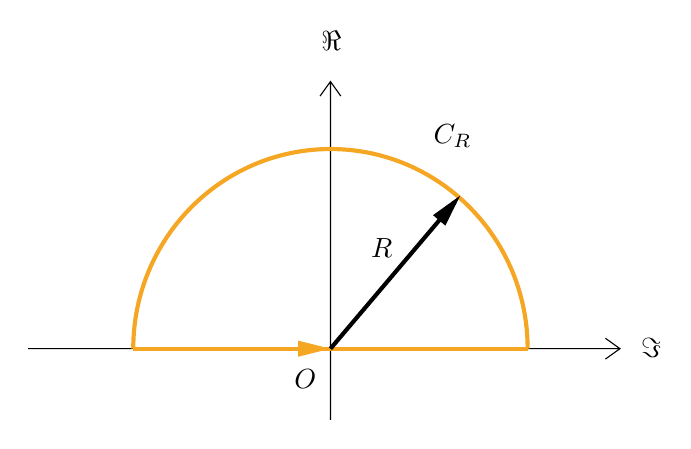
\begin{tikzpicture}[x=0.75pt,y=0.75pt,yscale=-1,xscale=1]
%uncomment if require: \path (0,266); %set diagram left start at 0, and has height of 266

%Shape: Axis 2D [id:dp1282392211894816] 
\draw  (162,181.79) -- (447.09,181.79)(307.61,53.09) -- (307.61,216.09) (440.09,176.79) -- (447.09,181.79) -- (440.09,186.79) (302.61,60.09) -- (307.61,53.09) -- (312.61,60.09)  ;
%Shape: Arc [id:dp1814309272431356] 
\draw  [draw opacity=0][line width=1.5]  (212.6,181.79) .. controls (212.6,181.79) and (212.6,181.79) .. (212.6,181.79) .. controls (212.6,128.66) and (255.14,85.6) .. (307.61,85.6) .. controls (360.08,85.6) and (402.61,128.66) .. (402.61,181.79) -- (307.61,181.79) -- cycle ; \draw  [color={rgb, 255:red, 245; green, 166; blue, 35 }  ,draw opacity=1 ][line width=1.5]  (212.6,181.79) .. controls (212.6,181.79) and (212.6,181.79) .. (212.6,181.79) .. controls (212.6,128.66) and (255.14,85.6) .. (307.61,85.6) .. controls (360.08,85.6) and (402.61,128.66) .. (402.61,181.79) ;  
%Straight Lines [id:da15038694853465828] 
\draw [color={rgb, 255:red, 245; green, 166; blue, 35 }  ,draw opacity=1 ][line width=1.5]    (212.6,181.79) -- (402.61,181.79) ;
\draw [shift={(307.61,181.79)}, rotate = 180] [fill={rgb, 255:red, 245; green, 166; blue, 35 }  ,fill opacity=1 ][line width=0.08]  [draw opacity=0] (15.6,-3.9) -- (0,0) -- (15.6,3.9) -- cycle    ;
%Straight Lines [id:da12449754393780421] 
\draw [color={rgb, 255:red, 0; green, 0; blue, 0 }  ,draw opacity=1 ][line width=1.5]    (307.61,181.79) -- (352.62,128.69) -- (367.5,111.14) ;
\draw [shift={(370.09,108.09)}, rotate = 130.29] [fill={rgb, 255:red, 0; green, 0; blue, 0 }  ,fill opacity=1 ][line width=0.08]  [draw opacity=0] (15.6,-3.9) -- (0,0) -- (15.6,3.9) -- cycle    ;


% Text Node
\draw (289,190.4) node [anchor=north west][inner sep=0.75pt]    {$O$};
% Text Node
\draw (302,27.4) node [anchor=north west][inner sep=0.75pt]    {$\Re $};
% Text Node
\draw (456,175.4) node [anchor=north west][inner sep=0.75pt]    {$\Im $};
% Text Node
\draw (326,127.4) node [anchor=north west][inner sep=0.75pt]    {$R$};
% Text Node
\draw (356,72.4) node [anchor=north west][inner sep=0.75pt]    {$C_{R}$};

% \draw   (239.6, 212.79) circle [x radius= 5, y radius= 5]  (234.6,212.79) -- (244.6,212.79)(239.6,207.79) -- (239.6,217.79) ;
% \draw   (334.61, 116.6) circle [x radius= 5, y radius= 5]  (329.61,116.6) -- (339.61,116.6)(334.61,111.6) -- (334.61,121.6) ;
% \draw   (429.61, 212.79) circle [x radius= 5, y radius= 5]  (424.61,212.79) -- (434.61,212.79)(429.61,207.79) -- (429.61,217.79) ;
% \draw   (396.48, 139.8) circle [x radius= 5, y radius= 5]  (391.48,139.8) -- (401.48,139.8)(396.48,134.8) -- (396.48,144.8) ;
\end{tikzpicture}


\begin{figure}[htb!]
    \centering
    


\tikzset{every picture/.style={line width=0.75pt}} %set default line width to 0.75pt        

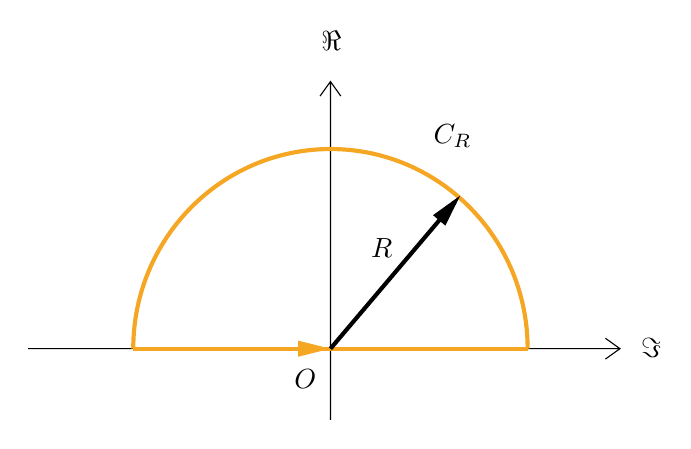
\begin{tikzpicture}[x=0.75pt,y=0.75pt,yscale=-1,xscale=1]
%uncomment if require: \path (0,266); %set diagram left start at 0, and has height of 266

%Shape: Axis 2D [id:dp1282392211894816] 
\draw  (162,181.79) -- (447.09,181.79)(307.61,53.09) -- (307.61,216.09) (440.09,176.79) -- (447.09,181.79) -- (440.09,186.79) (302.61,60.09) -- (307.61,53.09) -- (312.61,60.09)  ;
%Shape: Arc [id:dp1814309272431356] 
\draw  [draw opacity=0][line width=1.5]  (212.6,181.79) .. controls (212.6,181.79) and (212.6,181.79) .. (212.6,181.79) .. controls (212.6,128.66) and (255.14,85.6) .. (307.61,85.6) .. controls (360.08,85.6) and (402.61,128.66) .. (402.61,181.79) -- (307.61,181.79) -- cycle ; \draw  [color={rgb, 255:red, 245; green, 166; blue, 35 }  ,draw opacity=1 ][line width=1.5]  (212.6,181.79) .. controls (212.6,181.79) and (212.6,181.79) .. (212.6,181.79) .. controls (212.6,128.66) and (255.14,85.6) .. (307.61,85.6) .. controls (360.08,85.6) and (402.61,128.66) .. (402.61,181.79) ;  
%Straight Lines [id:da15038694853465828] 
\draw [color={rgb, 255:red, 245; green, 166; blue, 35 }  ,draw opacity=1 ][line width=1.5]    (212.6,181.79) -- (402.61,181.79) ;
\draw [shift={(307.61,181.79)}, rotate = 180] [fill={rgb, 255:red, 245; green, 166; blue, 35 }  ,fill opacity=1 ][line width=0.08]  [draw opacity=0] (15.6,-3.9) -- (0,0) -- (15.6,3.9) -- cycle    ;
%Straight Lines [id:da12449754393780421] 
\draw [color={rgb, 255:red, 0; green, 0; blue, 0 }  ,draw opacity=1 ][line width=1.5]    (307.61,181.79) -- (352.62,128.69) -- (367.5,111.14) ;
\draw [shift={(370.09,108.09)}, rotate = 130.29] [fill={rgb, 255:red, 0; green, 0; blue, 0 }  ,fill opacity=1 ][line width=0.08]  [draw opacity=0] (15.6,-3.9) -- (0,0) -- (15.6,3.9) -- cycle    ;


% Text Node
\draw (289,190.4) node [anchor=north west][inner sep=0.75pt]    {$O$};
% Text Node
\draw (302,27.4) node [anchor=north west][inner sep=0.75pt]    {$\Re $};
% Text Node
\draw (456,175.4) node [anchor=north west][inner sep=0.75pt]    {$\Im $};
% Text Node
\draw (326,127.4) node [anchor=north west][inner sep=0.75pt]    {$R$};
% Text Node
\draw (356,72.4) node [anchor=north west][inner sep=0.75pt]    {$C_{R}$};

% \draw   (239.6, 212.79) circle [x radius= 5, y radius= 5]  (234.6,212.79) -- (244.6,212.79)(239.6,207.79) -- (239.6,217.79) ;
% \draw   (334.61, 116.6) circle [x radius= 5, y radius= 5]  (329.61,116.6) -- (339.61,116.6)(334.61,111.6) -- (334.61,121.6) ;
% \draw   (429.61, 212.79) circle [x radius= 5, y radius= 5]  (424.61,212.79) -- (434.61,212.79)(429.61,207.79) -- (429.61,217.79) ;
% \draw   (396.48, 139.8) circle [x radius= 5, y radius= 5]  (391.48,139.8) -- (401.48,139.8)(396.48,134.8) -- (396.48,144.8) ;
\end{tikzpicture}


    \caption{半圆路径.}
    \label{fig:semicircle}
\end{figure}
下面证明上式第二项为零.一般的对于任意$\theta_1 \leq \theta \leq \theta_2$, 
有$\lim_{R\to \infty} zf(z) = 0$,可以证明对于该角度对应的圆弧$C$有,
\begin{equation}
    \lim_{R \rightarrow \infty} \int_C f(z) dz = 0 .
\end{equation}

\[
    \begin{aligned}
    \lim _{R \rightarrow \infty}\left|\int_C f(z) d z\right| \leq \int_{\theta_1}^{\theta_2} \lim _{R \rightarrow \infty}\left|f\left(R e^{i \theta}\right) i R e^{i \theta}\right| & d \theta \\
    & \leq\left(\theta_2-\theta_1\right) \lim _{R \rightarrow \infty}\left|f\left(R e^{i \theta}\right) R e^{i \theta}\right|=0 .
    \end{aligned}
\]
也就是说,
\begin{equation}
    \int_{-R}^R f(x) d x = 2\pi \imath  \sum_{z_j\in \textrm{上半平面}} \Res f(z_j),
\end{equation}

\begin{example}
    计算\[ 
    I = \int_{-\infty}^{\infty} \frac{dx}{1 + x^2}   .
    \]
\end{example}
\begin{solution}
    由$f(z) = \frac{1}{1+ x^2} = \frac{1}{(z-\imath)(z+\imath)}$可知
    其单极点$\pm \imath$,其中$\imath$在上半平面.
    \[
      \Res f(+\imath) = \frac{1}{2\imath}  
    \]
    因此,$I = 2\pi \imath  \frac{1}{2\imath} = \pi$.由于该积分是一个常见积分
    亦可以通过原函数$\arctan(x)$得到.留数定理的还可以计算这样的积分,
    \[
      I\int_{-\infty}^{\infty} \frac{dx}{(1 + x^2)^n} 
    \]
    具体求解过程参考梁昆淼数学物理方法的解.
\end{solution}


 \subsection{带复指数的定积分}
 考虑以下类型的定积分
 \begin{equation}
    I=\int_{-\infty}^{\infty} f(x) e^{\imath m x} d x
\end{equation}
其中,$m$为正实数;$f(z)$在上半平面除有限个奇点外是解析的,且$\lim_{|z|\to \infty} f(z) = 0, 0 \leq arg z \leq \pi$.
我们使用同样的半圆路径,类似的可以通过留数定理将实轴的积分转换为环路积分求得.
为了使用留数定理,我们先需要证明在半圆上的路径积分为零,这里就要用到\textbf{约旦引理}(Jordan lemma
).
即证明
\begin{equation}
    \lim _{R \rightarrow \infty} \int_{C_R} f(z) e^{\imath m z} d z=0 .
\end{equation}
当$R$足够大时,我们有$|f(z)| < \epsilon$.半圆积分
\begin{align}
    I_R&=\int_0^\pi f\left(R e^{\imath \theta}\right) 
    e^{\imath m R \cos \theta- m R \sin \theta} \imath R e^{\imath \theta} d \theta
    \\
    &\leq \epsilon R \int_0^\pi e^{-m R \sin \theta} d \theta=2 \epsilon R \int_0^{\pi / 2} e^{-m R \sin \theta} d \theta,
\end{align}
可以发现在$\left[ 0, \pi/2\right]$时,
\begin{equation}
    \frac{2}{\pi}\theta \leq \sin{\theta},
\end{equation}
于是有
\begin{equation}
    I_R \leq 2 \epsilon R \int_0^{\pi / 2} e^{-2 m R \theta / \pi} d \theta=2 \epsilon R \frac{1-e^{-m R}}{2 m R / \pi}<\frac{\pi}{m} \epsilon
\end{equation}
即
\begin{equation}
    \lim_{R\to \infty} I_R = 0.
\end{equation}
回到定积分$I$,可以得
\begin{equation}
    \label{eq:complex_exponential_integral}
    I=\int_{-\infty}^{\infty} f(x) e^{ \imath m x} d x = 2\pi \imath \sum_{z_j \in \text{上半平面}} \Res e^{\imath m z_j} f(z_j)
\end{equation}

对于以下类型的积分,可以利用上述结论.如
\begin{equation}
    \int_{0}^{\infty} f(x) \cos {m x} dx, \int_{0}^{\infty} G(x) \sin{m x} dx
\end{equation}
其中,$F(z)$为偶函数,$G(z)$为奇函数,它们在实轴上没有奇点,上半平面上除有限个奇点外解析.
很容易通过$\cos{mx} = \frac{1}{2}\left( e^{\imath m x} + e^{-\imath mx}\right)$等变换得到,即
$$
\begin{aligned}
\int_0^{\infty} F(x) \cos m x d x & =\int_0^{\infty} F(x) \frac{1}{2}\left(e^{\imath m x}+e^{-\imath m x}\right) d x \\
& =\frac{1}{2} \int_0^{\infty} F(x) e^{\imath m x} d x+\frac{1}{2} \int_0^{\infty} F(x) e^{-\imath m x} d x 
\\
& = \frac{1}{2} \int_{-\infty}^{\infty} F(x) e^{\imath m x} d x. 
\end{aligned}
$$

\begin{example}
计算 $\int_0^{\infty} \frac{\cos m x}{x^2+a^2} d x$.
\end{example}
\begin{solution}
偶函数$F(z) e^{\imath m z}=\frac{1}{z^2+a^2} e^{\imath m z}$ 有两个单极点 $\pm a \imath$, 其中 $+a \imath$ 在上半平面. 而 $e^{\imath m z} /\left(z^2+a^2\right)$ 在单极点 $+a \imath$ 的留数为
    $$
    \lim _{z \rightarrow a \imath}\left[(z-a \imath) \frac{e^{\imath m z}}{z^2+a^2}\right]=\lim _{z \rightarrow a \imath}\left[\frac{e^{\imath m z}}{z+a \imath}\right]=\frac{e^{-m a}}{2 a \imath}
    $$
    应用\eqref{eq:complex_exponential_integral},
    $$
    \int_0^{\infty} \frac{\cos m x}{x^2+a^2} d x=\pi \imath \frac{e^{-m a}}{2 a \imath}=\frac{\pi}{2 a} e^{-m a}.
    $$
\end{solution}
\section{Feynman技巧}
我们将讨论下面几个计算定积分的技巧.

\subsection{复变量代换}
以一个例子说明复变量代换的方法.求解定积分
\[
    I =  \int_0^{\infty} e^{-a x} \cos b x d x \\
\]
利用$\cos{bx} = \frac{1}{2}\left( e^{\imath b x} + e^{-\imath bx}\right)$
\[    \begin{aligned}
    I= & \frac{1}{2} \int_{0}^{\infty} \left(e^{-(a-\imath b) x} + e^{-(a + \imath b) x} \right)  d x \\
    = & \frac{1}{2} \left( \frac{1}{a-\imath b} +  \frac{1}{a+\imath b} \right)\\
    = & \frac{a}{a^2+b^2}
\end{aligned}
\]

\subsection{参数微分}
求解定积分
\[
    I =  \int_0^{\infty} x e^{-a x} \cos b x d x \\
\]
我们令
\[
  S(a) =   \int_0^{\infty} e^{-a x} \cos b x d x 
\]
已知 $S(a) = \frac{a}{a^2+b^2}$,通过对$S(a)$对$a$的求导得到
\[
    I = - S'(a)  = \frac{a^2 - b^2}{(a^2 +b^2)^2}    
\]
对于一般的含参数的微分,我们有
\begin{equation}
    \begin{aligned}
    \frac{d}{d \alpha} \int_{x_1(\alpha)}^{x_2(\alpha)} f(x, \alpha) d x= & \int_{x_1}^{x_2} \frac{\partial}{\partial \alpha} f(x, \alpha) d x \\
    & \left[\frac{d x_2(\alpha)}{d \alpha} \right] f(x_2, \alpha)- 
    \left[\frac{d x_1(\alpha)}{d \alpha}\right] f(x_1, \alpha)
    \end{aligned}
\end{equation}

\subsection{被积函数添加函数因子}
求解定积分
\[
    I =  \int_0^{\infty} \frac{\sin{x}}{x} d x 
\]
可以通过乘以一个函数因子$e^{-a x}$来构造参数函数
\[
 S(a) =     \int_0^{\infty}  e^{-a x} \frac{\sin{x}}{x} d x 
\]
这样我们有
\[
  S'(a) = -  \int_0^{\infty}  e^{-a x} \sin{x} d x  = \frac{1}{1+a^2}
\]
对于$a \to \infty$, 有 $S(\infty) = 0$.
而$\frac{1}{1+x^2}$的原函数为$\arctan{x}$,因此
\[S(a) = - \arctan{a} + C\]
可确定$C = \frac{\pi}{2}$,因此我们有$S(a) = \frac{\pi}{2} - \arctan{\alpha}$.
因此,
\[
  I = S(0) = \frac{\pi}{2} .    
\]
该结果我们已通过留数定理求得.
\section{积分求解实例}

\begin{itemize}
    \item 计算定积分 
    $$
    I=\int_0^{\infty} x^{\alpha-1} \frac{1}{1+x} d x \quad(0<\alpha<1).
    $$

    解 将被积函数 $x^{\alpha-1} /(1+x)$ 从实轴延拓到复数 $z$ 平面得到 
    $f(z)=z^{\alpha-1} /(1+z)$. 由于 $f(z)$ 含 有 $z^{\alpha-1}$ ,
    而 $\alpha$ 不是整数,所以 $f(z)$ 是多值函数, 它有两个支点:原点和无限远点. 
    $z$ 每绕原点或 无限远点一圈, 辐角增加 $2 \pi, z^{\alpha-1}$ 多出因子 
    $e^{\imath 2 \pi(\alpha-1)}$ 亦即 $e^{\imath 2 \pi \alpha}$,
     从而 $f(z)$ 也多出这么一个 因子.
    从原点沿着正实轴直至无限远作割线.   
    
    $$
\oint_l f(z) d z=\int_{\epsilon}^R \frac{x^{\alpha-1}}{1+x} d x+\int_{C_R} f(z) d z+\int_R^{\epsilon} \frac{x^{\alpha-1} e^{\imath 2 \pi \alpha}}{1+x} d x+\int_{C_{\epsilon}} f(z) d z .
$$
令 $R \rightarrow \infty, \epsilon \rightarrow 0$.
 上式左边按照留数定理应为 $2 \pi i\{f(z)$ 在有限远各奇点留数之和\}
  右边第一个积分成为所求的 $I$, 第三个积分则成为 $-e^{\imath 2 \pi \alpha} I$. 
  可以证明第 二个和第四个积分则成为零. 事实上,
  $$
\begin{aligned}
\left|\int_{C_R} \frac{z^{\alpha-1}}{1+z} d z\right| & =\left|\int_{C_R} \frac{z^\alpha}{1+z} \frac{d z}{z}\right| \leqslant \max _{\left(C_R \text { 上 }\right)}\left|\frac{z^\alpha}{1+z}\right| \frac{\int|d z|}{|z|} \\
= & \max \frac{R^\alpha}{|1+z|} \cdot \frac{2 \pi R}{R}=2 \pi \max \frac{R^\alpha}{|1+z|} \\
& \sim 2 \pi \frac{1}{R^{1-\alpha} \rightarrow 0} \quad(\text { 于 } R \rightarrow \infty) .
\end{aligned}
$$

$$
\begin{aligned}
\left|\int_{C_{\epsilon}} \frac{z^{\alpha-1}}{1+z} d z\right|= & \left|\int_{C_{\epsilon}} \frac{z^\alpha}{1+z} \frac{d z}{z}\right| \leqslant \max _{\left(C_{\epsilon} \text { 上 }\right)}\left|\frac{z^\alpha}{1+z}\right| \frac{\int|d z|}{|z|} \\
= & \max \frac{\epsilon^\alpha}{|1+z|} \cdot \frac{2 \pi \epsilon}{\epsilon}=2 \pi \max \frac{\epsilon^\alpha}{|1+z|} \\
& \sim 2 \pi \frac{\epsilon^\alpha}{1} \rightarrow 0 \quad(\text { 于 } \epsilon \rightarrow 0) .
\end{aligned}
$$
于是 $\left(1-e^{\imath 2 \pi \alpha}\right) I=2 \pi \imath\{f(z)$ 在有限远各奇点留数之和 $\}$.
$f(z)=z^{\alpha-1}(1+z)^{-1}$ 只有一个单极点 $z_0=-1=e^{\imath \pi}$, 而
$$
\Res f(-1)=\lim _{z \rightarrow-1}[(z+1) f(z)]=\lim _{z \rightarrow-1}\left[z^{\alpha-1}\right]=e^{\imath(\alpha \pi-\pi)}=-e^{\imath \alpha \pi} \text {. }
$$
因此
$$
\begin{aligned}
I & =-\frac{2 \pi \imath e^{\imath \pi \alpha}}{1-e^{\imath 2 \pi \alpha}}=-\frac{2 \pi \imath e^{\imath \pi \alpha}}{e^{\imath \pi \alpha}\left(e^{-\imath \pi \alpha}-e^{\imath \pi \alpha}\right)} \\
& =\frac{2 \pi \imath}{\left(e^{-\imath \pi \alpha}-e^{\imath \pi \alpha}\right)}=\frac{2 \pi \imath}{2 \sin \pi \alpha}=\frac{\pi}{\sin \pi \alpha} .
\end{aligned}
$$

    \item 计算菲涅耳积分(Fresnel integrals)
    $$
    I_1=\int_0^{\infty} \sin \left(x^2\right) \mathrm{d} x \text { 及 } I_2=\int_0^{\infty} \cos \left(x^2\right) \mathrm{d} x \text {. }
    $$

    解 由于 $\sin \left(x^2\right)=\operatorname{Im} e^{\imath x^2}$, 而 $\cos \left(x^2\right)=\operatorname{Re} e^{\imath x^2}$, 所以
$$
I_2+\imath I_1=\int_0^{\infty} e^{\imath x^2} d x .
$$
取图 4-10 所示回路 $l$. 由于 $e^{\mathrm{iz}^2}$ 没有有限远奇点, 所以根据留数定理得
$$
\oint_l e^{\imath z^2} d z=0,
$$
即 $\int_0^R e^{\imath x^2} d x+\int_{C_R} e^{\imath z^2} d z+\int_R^0 e^{\imath\left(\rho e^{\imath \pi / 4}\right)^2} d\left(\rho e^{\imath \pi / 4}\right)=0$,

令 $R \rightarrow \infty$. 第一个积分即所求的 $I_2+\imath I_1$. 第三个积分不难如下算出 :
$$
\begin{aligned}
\lim _{R \rightarrow \infty} \int_R^0 e^{\imath\left(\rho^2 \imath\right)} e^{\imath \pi / 4} d \rho & =\lim _{R \rightarrow \infty}\left(-e^{\imath \pi / 4}\right) \int_0^R e^{-\rho^2} d \rho=-e^{\imath \pi / 4} \int_0^{\infty} e^{-\rho^2} d \rho \\
& =-\frac{\sqrt{\pi}}{2} e^{\imath \pi / 4}=-(1+\imath) \sqrt{\frac{\pi}{8}} .
\end{aligned}
$$
可以证明第二个积分成为零. 为此, 先作一次分部积分,
$$
\int_{C_R} e^{\imath z^2} d z=\left.\frac{e^{\imath z^2}}{2 \imath z}\right|_{z=R} ^{R e^{\imath \pi / 4}}+\int_{C_R} e^{\imath z^2} \frac{\mathrm{d} z}{2 \imath z^2},
$$
其中已积出部分的模
$$
\left|\frac{e^{-R^2}}{2 \imath R e^{\imath \pi / 4}}-\frac{e^{\imath R^2}}{2 \imath R}\right| \leqslant \frac{e^{-R^2}}{2 R}+\frac{1}{2 R} \rightarrow 0 \quad(\text { 于 } R \rightarrow \infty),
$$
未积出部分的模
$$
\begin{aligned}
\left|\int_{C_R} \frac{e^{\imath 2^2}}{2 \imath {z}^2} d z\right| & =\left|\int_{C_R} \frac{e^{-R^2 \sin 2 \varphi+\imath^2 \cos 2 \varphi}}{2 \imath R^2 e^{\imath 2 \varphi}} R e^{\imath \varphi} \imath d \varphi\right| \\
& \leqslant \int_{C_R} \frac{e^{-R^2 \sin 2 \varphi}}{2 R^2} R d \varphi \leqslant \max \left(\frac{e^{-R^2 \sin 2 \varphi}}{2 R}\right) \frac{\pi}{4}
\\
&=\frac{1}{2 R} \frac{\pi}{4} \rightarrow 0 \quad(\text { 于 } R \rightarrow \infty) .
\end{aligned}
$$
于是
$$
\begin{gathered}
I_2+\imath I_1-\sqrt{\frac{\pi}{8}}(1+\imath)=0, \\
I_1=\sqrt{\frac{\pi}{8}}, \quad I_2=\sqrt{\frac{\pi}{8}} .
\end{gathered}
$$
\item 考虑用Feynman技巧来计算
$$
I = \int_0^1 \frac{x^2-1}{\log x} d x
$$
设计这样的函数
$$
G(t):=\int_0^1 \frac{x^t-1}{\log x} d x
$$
$G(0) = 0$,于是问题变为求$G(2)$.不难验证
$$
G^{\prime}(t)=\int_0^1 x^t d x=\frac{1}{t+1}
$$
对$t$求积分后得到
$$
G(2)=\int_0^2 G^{\prime}(t) d t=\int_0^2 \frac{d t}{t+1}=\log 3.
$$

\item 考虑用Feynman技巧来验证高斯积分:
$$
\int_0^{\infty} e^{-x^2} d x = \frac{\sqrt{\pi}}{2}.
$$
\\
定义一个$t$的函数
$$
I(t):=\int_0^{\infty} \frac{e^{-x^2}}{1+(x / t)^2} d x, t>0. 
$$
于是菲涅尔积分就是求$I_1 = I(\infty)$.
做代换$x/t=y$后,并换回积分变量为$x$有 $$
I(t)=t \int_0^{\infty} \frac{e^{-t^2 x^2}}{1+x^2} d x
$$
可以得到 $$
\lim _{t \rightarrow 0} \frac{I(t)}{t}=\frac{\pi}{2}.
$$
为了能利用上面的技巧,我们将考虑
$$
e^{-t^2} I(t)=t \int_0^{\infty} \frac{e^{-t^2\left(1+x^2\right)}}{1+x^2} d x
$$
对于
$$
\frac{d}{d t}\left(t^{-1} e^{-t^2} I(t)\right)=\int_0^{\infty}-2 t e^{-t^2\left(1+x^2\right)} d x=-2 e^{-t^2} \int_0^{\infty} e^{-u^2} d u=-2 e^{-t^2} I(\infty)
$$

两边积分
$$
\underbrace{\int_0^{\infty} \frac{d}{d t}\left(t^{-1} e^{-t^2} I(t)\right) d t}_{=-\lim _{t \rightarrow 0} \frac{I(t)}{t}}=\underbrace{\int_0^{\infty}-2 e^{-t^2} I(\infty) d t}_{=-2 I(\infty)^2}
$$
得到
$$
I(\infty) = \sqrt{\frac{\pi}{4}} = \frac{\sqrt{\pi}}{2}.
$$

\end{itemize}
% \input{infinite_range.tex}


% \end{CJK}
\end{document}